%|  CSUS CPE64/EEE64 Verilog Labs: Lab Two
%|
%|  language: LaTeX
%|  Author: Ben Smith
%| 
%|  This source generates the lab manual document when compiled using a LaTeX processor.  All packages are included in a full
%|  installation of a LaTeX System.  
%|
%| 
%| 
\title{Lab Two: Introduction to logic on the FPGA}
\author{Ben Smith}
%| This is a header file for Latex documents  
%| It contains a number of common packages, settings, and custom macros that I frequently use.
\documentclass[9pt,journal]{IEEEtran}

\usepackage[cmex10]{amsmath}        %| American Mathematical Society package for fancy maths  b
\interdisplaylinepenalty=2500              %| Restores IEEE line spacing after amsmath

%| IEEE Citation package
\usepackage{cite}
\usepackage[section]{placeins}
\usepackage{array}
\usepackage{dblfloatfix}
\usepackage{color}
\usepackage{graphicx}
\usepackage{float}
\usepackage{url}                         %| Improved URL handling
\usepackage{etoolbox}
\usepackage[font=footnotesize]{subcaption}
\usepackage{listings}
\usepackage{fixltx2e}               %| Better tables than for LaTeX 2e
\usepackage{minted}

%| Highlighting for source code listings
\definecolor{mygreen}{rgb}{0,0.6,0}
\definecolor{ltgray}{rgb}{0.93,0.93,0.93}
\definecolor{dkgray}{rgb}{0.5,0.5,0.5}
\definecolor{mymauve}{rgb}{0.58,0,0.82}
\lstset{
  backgroundcolor=\color{ltgray},  % choose the background color; you must add \usepackage{color} or \usepackage{xcolor}
  basicstyle=\scriptsize\ttfamily, % the size of the fonts that are used for the code
  breakatwhitespace=true,         % sets if automatic breaks should only happen at whitespace
  breaklines=true,                 % sets automatic line breaking
  captionpos=b,                    % sets the caption-position to bottom
  commentstyle=\color{mygreen},    % comment style
  deletekeywords={...},            % if you want to delete keywords from the given language
  escapeinside={\%*}{*)},          % if you want to add LaTeX within your code
  extendedchars=true,              % lets you use non-ASCII characters; for 8-bits encodings only, does not work with UTF-8
  frame=single,                    % adds a frame around the code
  keepspaces=true,                 % keeps spaces in text, useful for keeping indentation of code (possibly needs columns=flexible)
  keywordstyle=\color{blue},       % keyword style
  language=SystemVerilog,          % the language of the code(I modified the .sty for systemverilog, found the code on google)
  morekeywords={*,...},            % if you want to add more keywords to the set
  numbers=left,                    % where to put the line-numbers; possible values are (none, left, right)
  numbersep=4pt,                   % how far the line-numbers are from the code
  numberstyle=\tiny\color{dkgray}, % the style that is used for the line-numbers
  rulecolor=\color{black},         % if not set, the frame-color may be changed on line-breaks within not-black text (e.g. comments (green here))
  showspaces=false,                % show spaces everywhere adding particular underscores; it overrides 'showstringspaces'
  showstringspaces=false,          % underline spaces within strings only
  showtabs=false,                  % show tabs within strings adding particular underscores
  stepnumber=2,                    % the step between two line-numbers. If it's 1, each line will be numbered
  stringstyle=\color{mymauve},     % string literal style
  tabsize=2,                       % sets default tabsize to 2 spaces
  title=\lstname                   % show the filename of files included with \lstinputlisting; also try caption instead of title
}

\lstset{keywordstyle=\color{purple}}
\lstset{keywordstyle={[2]\color{purple}} }
\lstset{keywordstyle={[3]\color{magenta}} }
\lstset{keywordstyle={[4]\color{teal} }}
\lstset{keywordstyle={[5]\color{violet!40}} }

% Alter some LaTeX defaults for better treatment of figures:
  % See p.105 of ''TeX Unbound'' for suggested values.
  % See pp. 199-200 of Lamport's ''LaTeX'' book for details.
  %   General parameters, for ALL pages:
  \renewcommand{\topfraction}{0.9}  % max fraction of floats at top
  \renewcommand{\bottomfraction}{0.8} % max fraction of floats at bottom
  %   Parameters for TEXT pages (not float pages):
  \setcounter{topnumber}{2}
  \setcounter{bottomnumber}{2}
  \setcounter{totalnumber}{4}     % 2 may work better
  \setcounter{dbltopnumber}{2}    % for 2-column pages
  \renewcommand{\dbltopfraction}{0.9} % fit big float above 2-col. text
  \renewcommand{\textfraction}{0.07}  % allow minimal text w. figs
  %   Parameters for FLOAT pages (not text pages):
  \renewcommand{\floatpagefraction}{0.7}  % require fuller float pages
  % N.B.: floatpagefraction MUST be less than topfraction !!
  \renewcommand{\dblfloatpagefraction}{0.7} % require fuller float pages

%| Enables PDF metadata, thumbnails, and navigation
\newcommand\MYhyperrefoptions{
  bookmarks=true,
  bookmarksnumbered=true,
  pdfpagemode={UseOutlines},
  plainpages=false,
  pdfpagelabels=true,
  colorlinks=true,
  linkcolor={black},
  citecolor={black},
  urlcolor={blue},
  pdftitle={CPE/EEE 64 Lab},
  pdfsubject={Engineering},                        
  pdfauthor={Ben Smith},
  pdfkeywords={Logic Design, FPGA, Verilog}}                       

%| Calls hyperref package with the options specified above
\usepackage[\MYhyperrefoptions,pdftex]{hyperref}

%| Font settings
\renewcommand{\sfdefault}{phv}
\renewcommand{\rmdefault}{ptm}
\renewcommand{\ttdefault}{pcr}

%| Restores IEEE table formatting after usage of subcaption package
\captionsetup[table]{format=plain,labelformat=simple,justification=centering, labelsep=newline, singlelinecheck=false, textfont={sc}}

%| Required Lab Demo custom function
%| \demo{Name}{Physical deliverable}{Documentation deliverable}{Process}
%| =================================================================================================
%| for boxed text and stuch
\usepackage{fancybox}
\newenvironment{fminipage}%
{\begin{Sbox}\begin{minipage}}%
{\end{minipage}\end{Sbox}\Ovalbox{\TheSbox}}

%| Actual bawx
\newcommand{\demo}[4] {
\vspace{15px}
\begin{centering}
  \begin{fminipage}{.47\textwidth}
    \vspace{3px}
    \centering{\bfseries \large Laboratory Demo: #1}\\*
    \vspace{10px}
    \begin{tabular}{p{1.4cm}  p{6.3cm}}
      %|==Requirements for lab demo==
      \raggedright Specification:                  &#2\\
      \\
      \raggedright  Deliverable:                   &#3\\
      \\
      \raggedright Process :                       &#4\\
    \end{tabular}
  \end{fminipage}
\end{centering}
}

%| Single figure
%| \small{Location}{Caption}{Label}
%| =================================================================================================
\newcommand{\smallfig}[3] {
  \begin{figure}[H]
    \includegraphics[width=.48\textwidth]{#1}
    \caption{#2}
    \label{#3}
  \end{figure}
}

%| Single figure
%| \simpletable{c||c}{Caption}{Label}{content}
%| =================================================================================================
\newcommand{\simpletable}[4] {
  \begin{table}[!t]
    \caption{#2}
    \label{#3}
    \centering
    \begin{tabular}{#1}
      \hline
      #4
    \end{tabular}
  \end{table}
}

\begin{document}
\maketitle

  \begin{abstract}
    This document is an introduction to the DE0-Nano development board, Altera's Cyclone IV FPGA and the Quartus IDE. The schematic editor feature of Quartus is used to synthesize logic gate primitives and more complex logic functions from these primitives. The synthesis of these simple structures allows the student to gain experience with the development tools used by the DE0-Nano Development board.
  \end{abstract}

  %| =================================================================================================
  %| Introduction
  %| =================================================================================================
  \section{Introduction}
    \PARstart{T}{he} first lab in this intraductory series introduces the DE0-Nano development board and Altera's Quartus development environment. Quartus will be used to program the Altera Cyclone IV FPGA on the Terasic DE0-Nano development board.\footnote{FPGAs remained a mystery to me for quite some time, the video does a great job of discussing the benefits and drawbacks of the devices \href{https://www.youtube.com/watch?v=gUsHwi4M4xE}{EEV Blog: What is a FPGA?}}  The schematic entry method used in this lab will be very similar to the design entry method that you have experienced with in first lab with Multisim. Now, instead of discrete logic, the FPGA will implement the logic. The Cyclone IV could implement the equivalent of 3300 2-input nand gates. Imagine hand wiring and the amount of circuit board space all that logic would require if using Discrete ICs. This lab is intended to introduce the student to the following concepts:
    \begin{itemize}
       \item Logic primitives on a FPGA
       \item Quartus development environment
       \item Synthesis of a block based design
       \item Assigning pins for a design
       \item Programming an Altera FPGA
    \end{itemize}

    \subsection{Included Screencasts}
      A number of screencasts are included with this set of labs. They are available on Youtube and as zipped MP4s on the course website. They are intended to be brief so they cover individual topics.
      \begin{enumerate}
        \item TIME - Installing Quartus
        \item TIME - Block editor in Quartus
      \end{enumerate}

    \subsection{DE0-Nano Development board}
      The DE0-Nano has a number of peripheral devices built into the board to expand the capabilities of the FPGA. Interacting with most of these devices will be beyond the scope of this course but represent real world design challenges and are worth experimenting with after this course is completed. Altera and Terasic offer a number of tutorials for the periphrial devices though in the \href{http://www.terasic.com.tw/cgi-bin/page/archive_download.pl?Language=English&No=593&FID=75023fa36c9bf8639384f942e65a46f3}{DE0-Nano user manual} and the Altera University Program. These labs will mostly use one of the 40-pin GPIO headers to interact with the outside world. Let's take a moment to recognise the potential of this development board should you choose to pursue it. Figure \ref{DEOBlockDia} shows a high level diagram of the development board. There is much more information available in the DE0-Nano manual but these are some system highlights. The SDRAM can be used to store large amounts of information for fast access, great for a {\it soft processor} \footnote{A soft processor is a microprocessor implemented inside of the FPGA. These softprocessors can be programmed in languages like C for more standard development processes that typically are much faster than HDL languages. The advantage of this method is the ability to build the microcontroller to suit a particular design and build hardware periphrials with the FPGA}. The EEPROM allows program memory that does not clear with power reset, also very useful for a soft processor. The A/D converter allows analog voltages to be read which allows the development board to interact with the outside world. It also features an accelerometer that will refresh at rates up to 1600Hz.      
      \begin{figure}[htpb]
        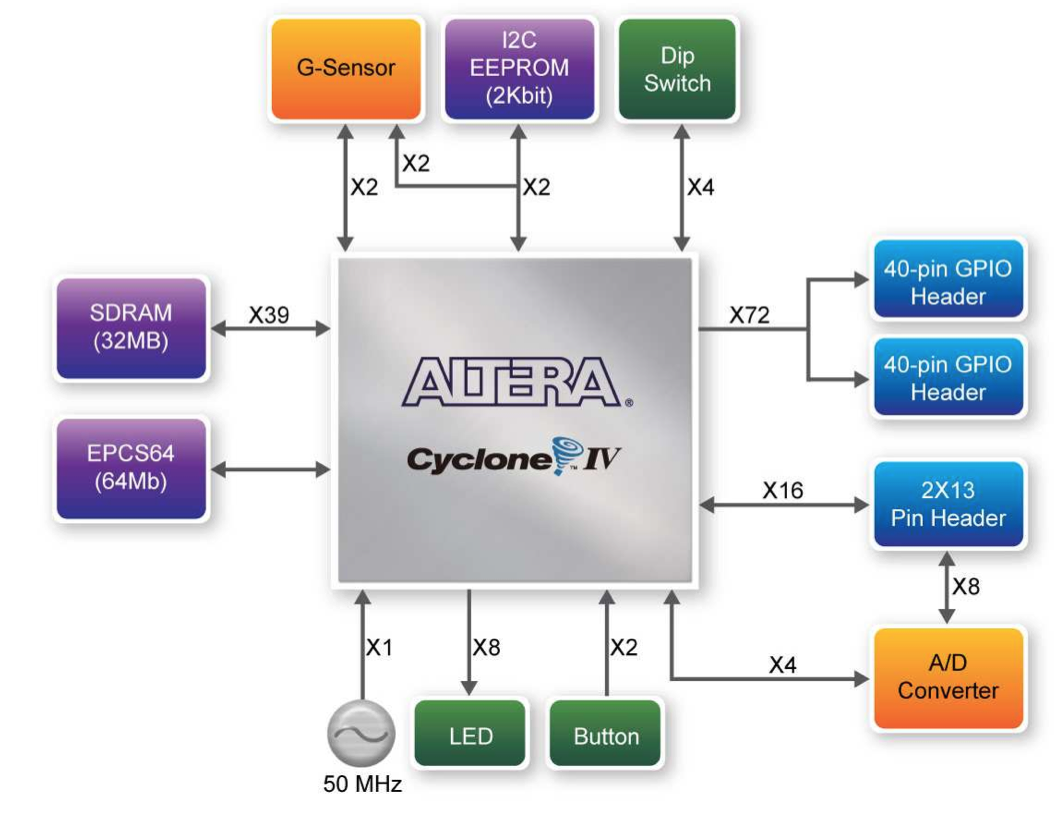
\includegraphics[width=.48\textwidth]{Images/DEONanoBlockDiagram.png}
        \caption{Block Diagram of DE0-Nano \cite{DE0Manual}}
        \label{DEOBlockDia}
      \end{figure}
      The A/D converter and G-sensor will be great tools to interact with sensors in your later classes. If you choose to go down a path of controls engineering FPGAs will be a great way to implement {\it deterministic}\footnote{a deterministic system is a system in which no randomness is involved in the development of future states of the system. A deterministic model will thus always produce the same output from a given starting condition or initial state.\cite{DynamicSystems}} Control systems. Interfacing with these periphrials will require the implementation of a bus protocal like SPI or I2C. The De0-Nano system CD comes with some example code that uses these devices that would get the interested student off the ground in no time.

  %| =================================================================================================
  %| Procedure
  %| =================================================================================================
  \section{Lab Procedure}
    \PARstart{T}{his} section is a guide for what must be accomplished in the lab. Keep in mind, the some of the following material will need to be documented in your lab report. It would behoove you to take a look at the lab report section before starting the procedure. Recording results of experiments will be stressed because the documentation of what you do is the most important part. To begin these labs you will need:
    \begin{itemize}
      \item De0-Nano Development board
      \item A breadboard
      \item Four LEDs with 200$\Omega$ current limiting resistors
      \item Two dip switches with 200$\Omega$ pulldown resistors
      \item Windows or Linux based computer
      \item Internets
    \end{itemize}
    
    %| Step One: Introduction to DE0-Nano Board
    %| =================================================================================================
    \subsection{Getting start with your DE0-Nano}
      Altera's University program provides excellent tutorials for Quartus. This first tutorial covers installation of drivers for the DE-Series board. This is information will only be pertenent to those installing quartus on their own computer. \href{http://www.altera.com/literature/manual/quartus_install.pdf}{Installing Quartus} 

    %| Step One: Introduction to Quartus
    %| =================================================================================================
    \subsection{Lab Part One: LED controller with onboard devices.}
      The included document \href{ftp://ftp.altera.com/up/pub/Altera_Material/13.0/Tutorials/Schematic/Quartus_II_Introduction.pdf}{Quartus II Introduction} shows how to use the graphical editor feature of quartus. Dont worry about section 8 of the Quartus Introduction, we'll cover simulators later. The product of this tutorial will be the first lab demo. Notice the Boxed section below, demos will be presented as a specification and deliverable format. This first Example box describes what the three sections mean and how to use this information to help you successfully demo the lab.

      \demo{Example 2-input NAND Gate}
          {The Specification will be a description of device behavior and a set of constraints for it's implementation. Assume all demos have the technology constraint of using the DE0-Nano. The specification for this example would be to implement a NAND gate with the onboard dip switches as inputs and the LEDs as outputs.}
          {The deliverable will always be the DEO0-Nano board with or without some associated circuitry}
          {The product of the specification is to be verified in some way during the laboratory peroid. This will involve demonstrating the design to instructor or one of the lab assistants.}

      \demo{Light Controller}
          {Use onboard periphrials to generate inputs for the FPGA to control an LED according to Figure 11 of the Altera tutorial {\it Quartus II Introduction.}}
          {Labeled schematic of circuit with I/O pins labeled with FPGA pin number and Verilog net name,  truth table from your  experimental result.}
          {The student will be asked the result of a few random numbers to verify the correct operation of their circuit.}

    %| Step Three: Prepare circuit
    %| =================================================================================================
    \subsection{Lab Part Two: Interacting with external devices though GPIO}
      A switch and LED are going to be used to test the FPGA while it's operating. This switch will allow you to generate input for the FPGA. Figure \ref{LEDCircuit} LED circuit needs a current limiting resistor.
      \begin{figure}[htpb]
        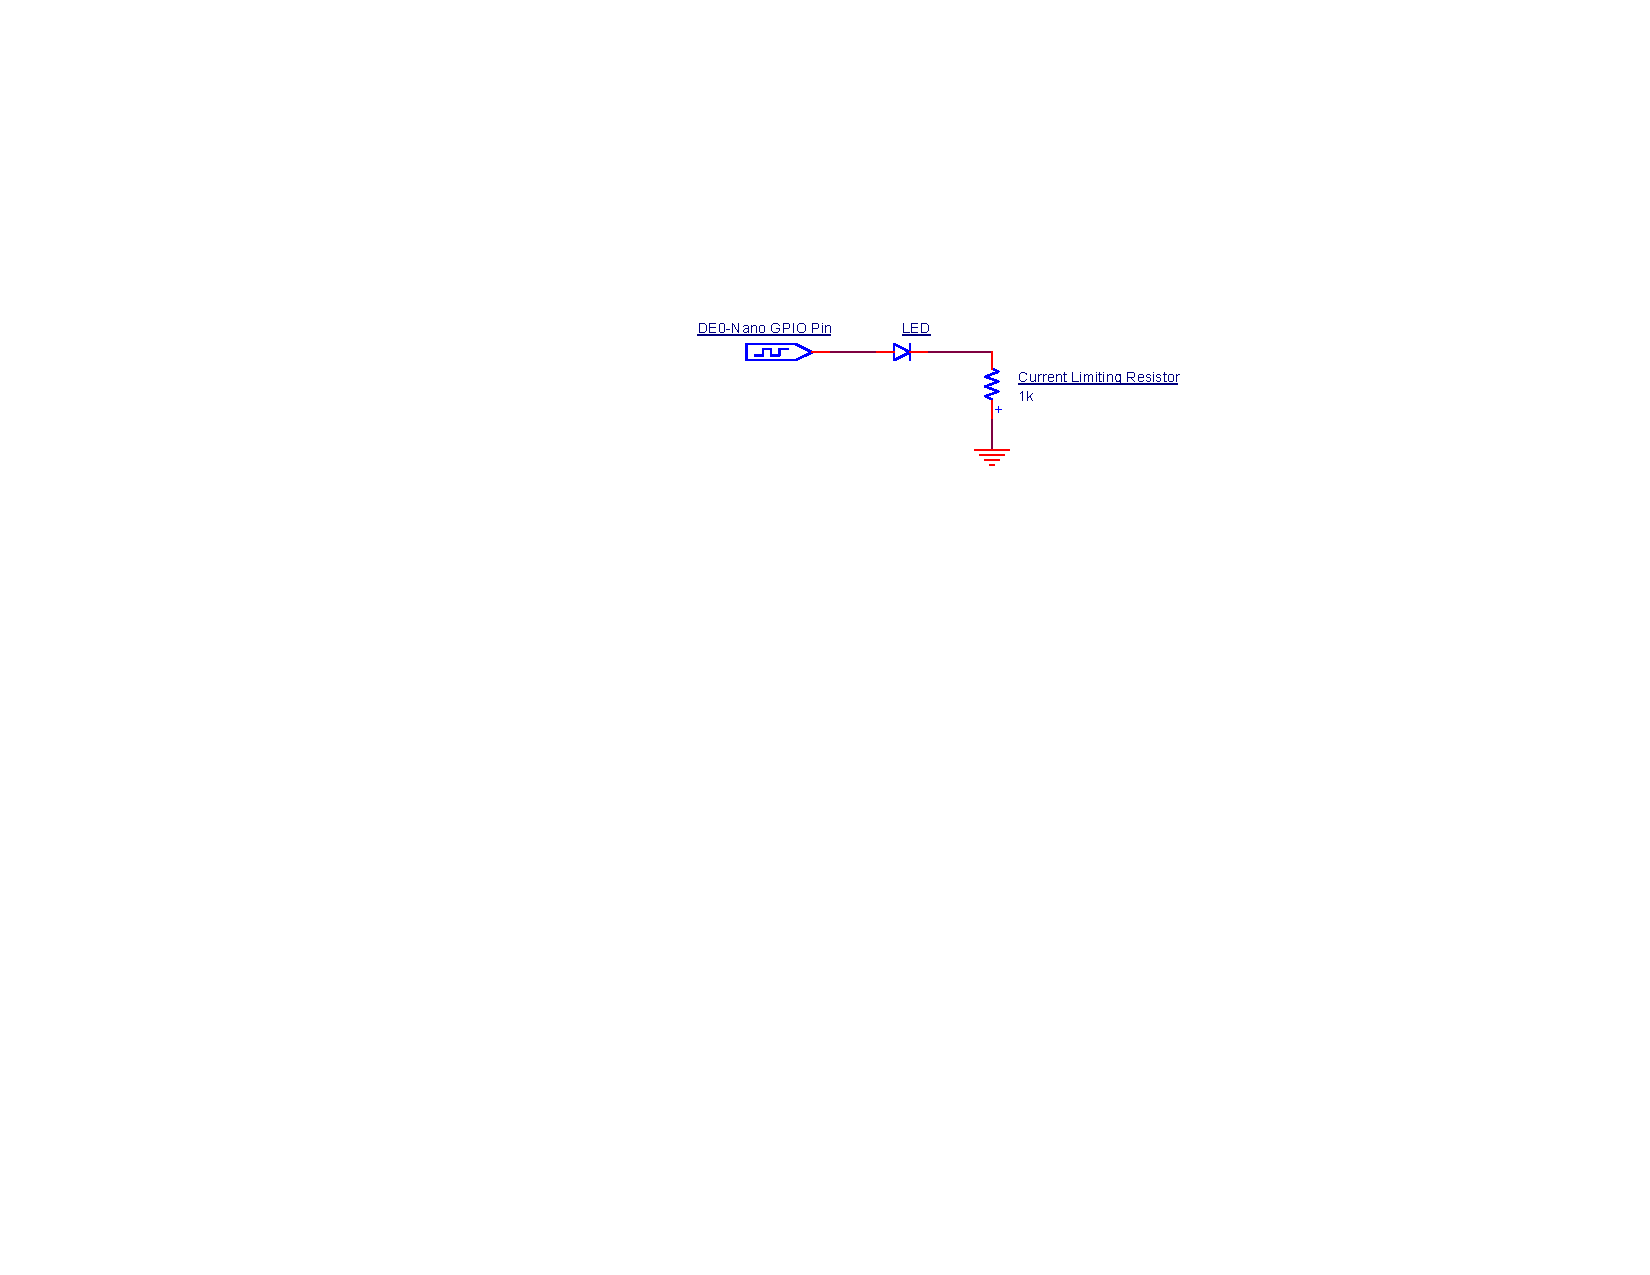
\includegraphics[width=.48\textwidth]{Schematics/LED.pdf}
        \caption{LED with current limiting resistor}
        \label{LEDCircuit}
      \end{figure}
      The LED will allow you to see the the output but we'll also need to be able to generate some input for the FPGA. We will do this with a dip switch and pulldown resistor. The pulldown resistor is needed to literally pull the charge off the wire so the input will read a solid zero. Otherwise the pin would {\it float} between 1 and 0 arbitrarily. CMOS devices tend to float to the high state, so if you ever have a signal stuck high, it's worth looking into the pulldown network if you're using one.

      \begin{figure}[htpb]
        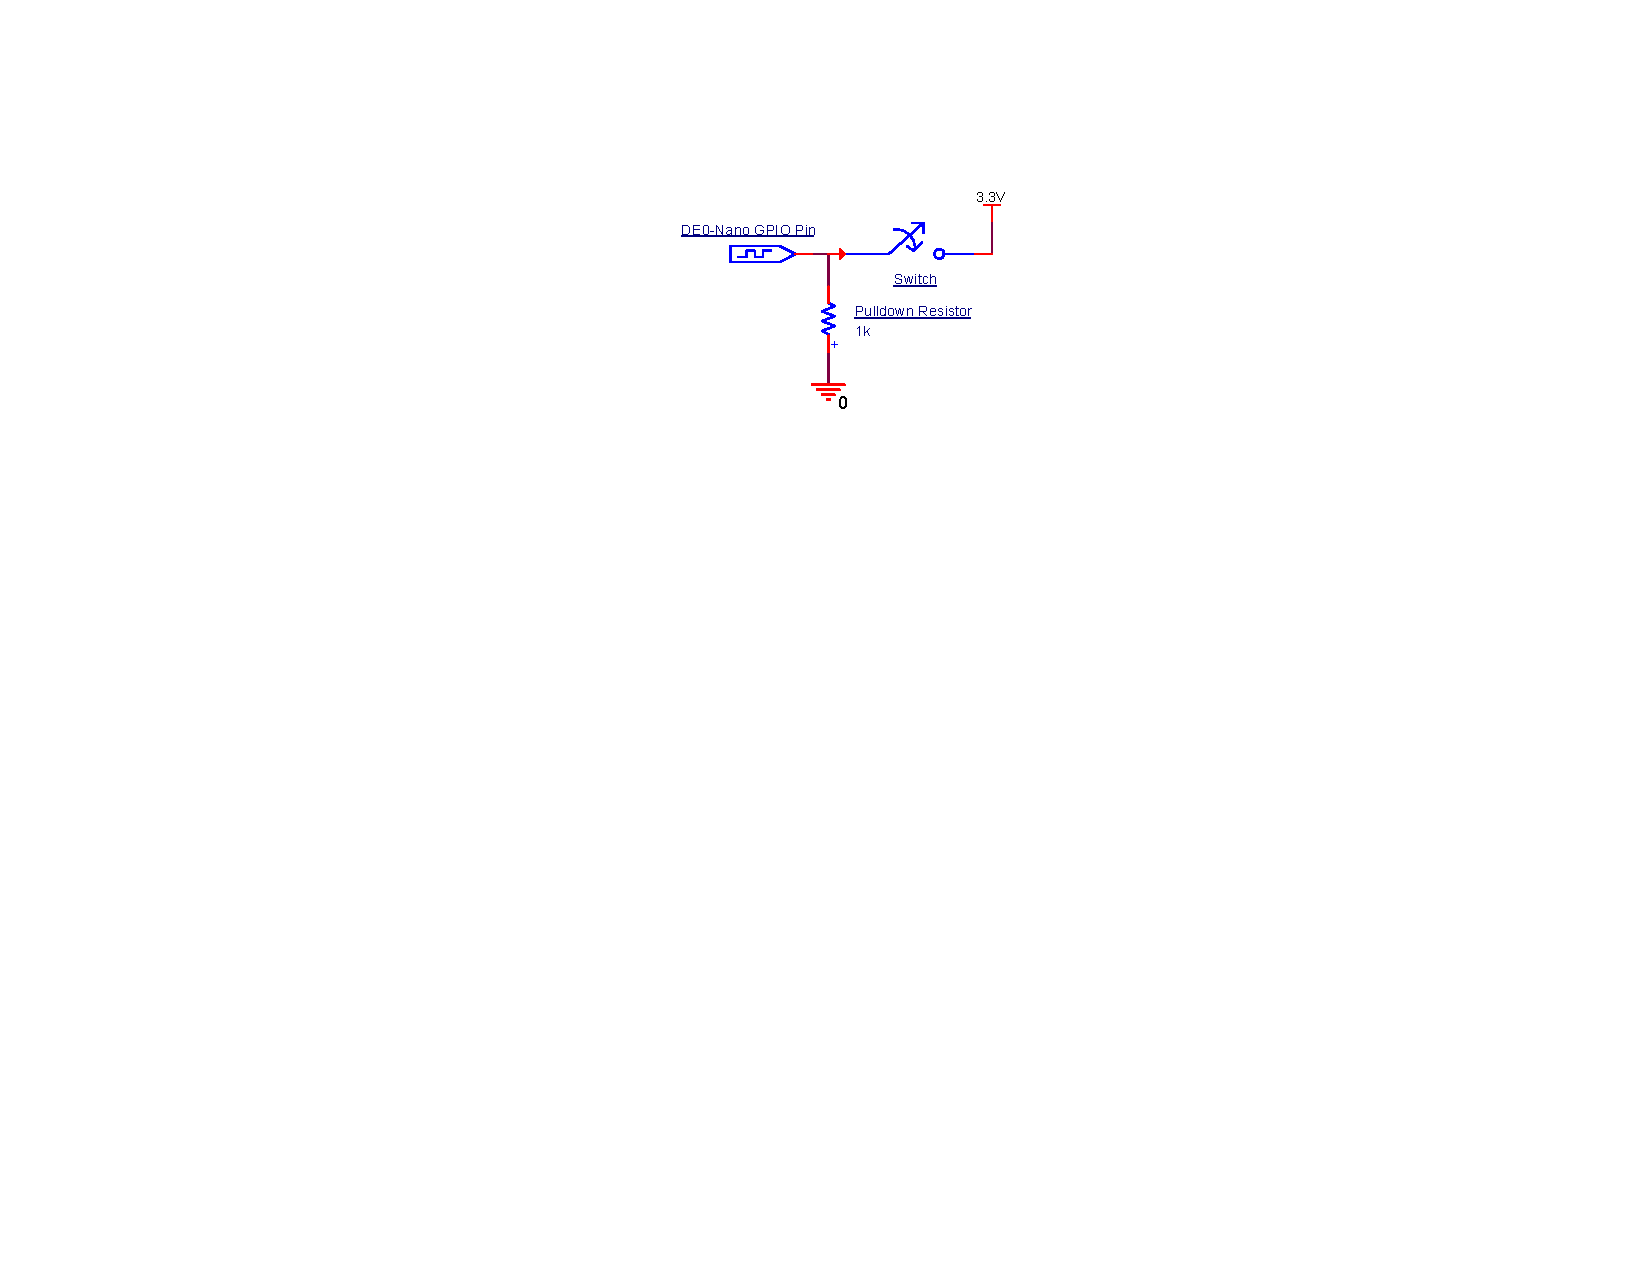
\includegraphics[width=.38\textwidth]{Schematics/SwitchCircuit.pdf}
        \caption{Switch with pulldown resistor}
        \label{swPulldown}
      \end{figure}

      %| GPIO Headers
      \subsubsection{GPIO headers on the DE0-Nano} 
        Be careful when referencing the pin diagrams in the DE0-Nano user manual. It is easy to read it backwards, a simple mistake like this can cost a sub stantial amount of time. It is easiest to match the Nano's orientation with the schematic and count from the nearest edge. Figure \ref{pinmap} shows GPIO 0 next to a schematic of the header. Always check VCC\_SYS, VCC3P3, and GND with a multimeter before attaching a circuit you have built.        
        \begin{figure*}
          \centering
          \begin{subfigure}[b]{.38\textwidth}
            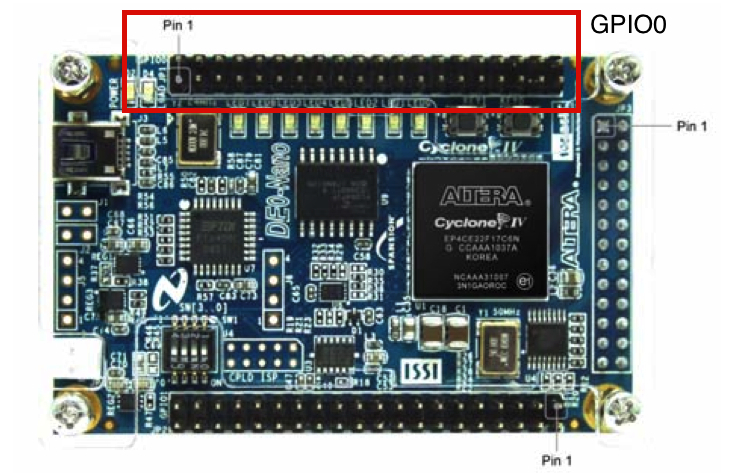
\includegraphics[angle=270, width=.9\textwidth]{Images/LabeledGPIOHeaders.jpg}
            \caption{Orientation of GPIO Header\cite{DE0Manual}}
          \end{subfigure}
          \begin{subfigure}[b]{.45\textwidth}
            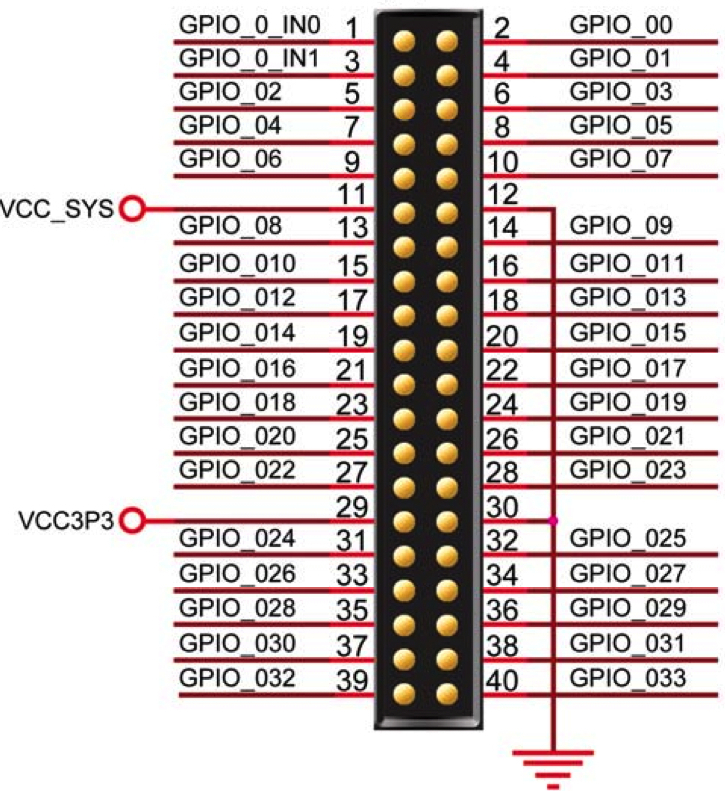
\includegraphics[width=\textwidth]{Images/GPIOHeader.jpg}
            \caption{Schematic of GPIO-0 header\cite{DE0Manual}}
          \end{subfigure}
          \caption{GPIO0 and its orientation on the development board}
          \label{pinmap}
        \end{figure*}
        This is the header pin schematic from the DE0-Nano user manual. Inside the Verilog code, these pins follow a different nomenclature. What is labeled as GPIO\_0\_IN[0] in figure 5 is GPIO0\_IN[0] and GPIO\_00 is GPIO0[0]. Refer to the DE0-Nano user guide for details on the orientation of the headers.        

      %| Step Eight: Create AOI module from equation
      %| =================================================================================================
      \subsection{Design AOI module from logical equation} 
        The {\it And or Invert} function is common in digital design. You will implement it with logic primitives in the schematic editor. There will be a wealth of information available online about how to implement the function on the Internet, but try and fail at least once before heading to Google.

      \begin{displaymath}
        F = \overline{(A \wedge B) \vee (C \wedge D)}
      \end{displaymath}

    %| Required Lab Demo
    %| =================================================================================================
    \demo{AOI Gate}
                  {4 dipswitch inputs and 1 LED outputs with appropriate pulldown and current limiting resistors for the DE0-Nano Development board. }
                  {Labeled schematic of circuit with I/O pins labeled with FPGA pin number and Verilog net name,  truth table from your  experimental result.}
                  {The student will be asked the result of a few random numbers to verify the correct operation of their circuit.}

  %| =================================================================================================
  %| Lab Report Requirements
  %| =================================================================================================
  \section{Lab Report}
    \IEEEPARstart{T}{he} lab report must be typed and submitted in a PDF format to the course's Moodle site. Look to \href{http://www.ieee.org/conferences_events/conferences/publishing/templates.html}{IEEE's guidelines} on format. I would reccomend  using the word template they provide, it will ensure professional looking documents without much effort. The document should include the following items.
    
    \subsection{Figures to include}
    \begin{itemize}
      \item Quartus schematic of your Light Controller module.
      \item Quartus Schematic of your AOI module.
      \item Truth tables for both designs.
    \end{itemize}

    \subsection{Questions to answer}
    \begin{enumerate}
      \item Notice the report that pops up when you compile your project. There are a number of statistics given by Quartus, the logic element usage ratio is your designs use of the total device capacity. What was the logic usage of your FPGA?
      \item The FPGA is based on 3.3 volt logic, what compataility issues do you anticipate with more common 5V devices like the 7400 series logic ICs you were using.
      \item This lab uses a graphical design entry method. What advantages do you see in this method, what drawbacks do you anticipate compared to a text based system?
    \end{enumerate}

  %| =================================================================================================
  %| Conclusion
  %| =================================================================================================
  \section{Conclusion}
    \IEEEPARstart{T}{this} lab introduced Quartus and some of it's basic functionality. Quartus is very similar to many industry standard tools. Xilinx, another manufacturer of programmable logic devices, offers a tool suite very similar to Quartus called ISE. Although we will not discuss ISE, an understanding of Quartus will allow ISE to be learned very quickly. These are tools that you can expect to see in Industry as a CPE or EEE student. There is an extreme demand right now for engineers with an understanding of programmable logic.

  %| =================================================================================================
  %| Bibliography
  %| =================================================================================================
  \bibliographystyle{IEEEtran}
\bibliography{IEEEfull}


\end{document}